%%# -*- coding:utf-8 -*-

\documentclass{article}
% if you need to pass options to natbib, use, e.g.:
%     \PassOptionsToPackage{numbers, compress}{natbib}
% before loading neurips_2022


% ready for submission
% \usepackage{neurips_2022}


% to compile a preprint version, e.g., for submission to arXiv, add add the
% [preprint] option:
%     \usepackage[preprint]{neurips_2022}

\PassOptionsToPackage{numbers, compress}{natbib}  % ref https://arxiv.org/abs/2209.09407
% to compile a camera-ready version, add the [final] option, e.g.:
\usepackage[final]{neurips_2022}

% to avoid loading the natbib package, add option nonatbib:
%    \usepackage[nonatbib]{neurips_2022}

% \usepackage[utf8]{inputenc} % allow utf-8 input
\usepackage[T1]{fontenc}    % use 8-bit T1 fonts
\usepackage{hyperref}       % hyperlinks
\usepackage{url}            % simple URL typesetting
\usepackage{booktabs}       % professional-quality tables
\usepackage{amsfonts}       % blackboard math symbols
\usepackage{nicefrac}       % compact symbols for 1/2, etc.
\usepackage{microtype}      % microtypography
\usepackage{xcolor}         % colors
\usepackage{graphicx}       %%  图片包
\usepackage{subfig}
\usepackage{geometry}
\usepackage{calligra}
\usepackage{algorithm}
\usepackage{algorithmicx}
\usepackage{algpseudocode} 
\usepackage{amsmath}
\usepackage{amssymb}
\usepackage{bm}
\usepackage{multirow}
\newtheorem{definition}{Definition}[section]
\newtheorem{theorem}{Theorem}[section]
\newtheorem{notations}{Notations}

\title{Reproduction of ``Fast and Accurate Matrix Completion via Truncated Nuclear Norm Regularization''}


% The \author macro works with any number of authors. There are two commands
% used to separate the names and addresses of multiple authors: \And and \AND.
%
% Using \And between authors leaves it to LaTeX to determine where to break the
% lines. Using \AND forces a line break at that point. So, if LaTeX puts 3 of 4
% authors names on the first line, and the last on the second line, try using
% \AND instead of \And before the third author name.


\author{%
  Zhao-Yang Liu\\ %\thanks{Use footnote for providing further information
    % about author (webpage, alternative address)---\emph{not} for acknowledging
    % funding agencies.} \\
    Sun Yat-sen University \\
  \texttt{liuzhy86@mail2.sysu.edu.cn} \\
  % examples of more authors
  \and
  Xin-Hua Zheng \\
  Sun Yat-sen University \\
  \texttt{zhengxh56@mail2.sysu.edu.cn} \\
  % \AND
  % Coauthor \\
  % Affiliation \\
  % Address \\
  % \texttt{email} \\
  % \And
  % Coauthor \\
  % Affiliation \\
  % Address \\
  % \texttt{email} \\
  % \And
  % Coauthor \\
  % Affiliation \\
  % Address \\
  % \texttt{email} \\
}


\begin{document}
{

\maketitle


\begin{abstract}
Recovering a large matrix from a small subset of its entries is a challenging problem arising in many real applications, such as computer vision. This can be considered as a low rank matrix approximation problem. If the nuclear norm is used as a convex relaxation of the rank operator, all singular values are minimized simultaneously by minimizing the nuclear norm, so the rank is not well approximated in practice. 
Yao Hu et al. proposed to achieve a better approximation to the rank of matrix by truncated nuclear norm, which is given by the nuclear norm subtracted by the sum of the largest few singular values. Furthermore, they developed a novel matrix completion algorithm and further developed three efficient iterative procedures TNNR-ADMM, TNNR-APGL and TNNR-ADMMAP to solve the optimization problem.
In this report, we reproduce the algorithm of Yao Hu et al. and related work, and perform experiments similar to their work. Our experiments show encouraging results of the algorithm proposed by Yao Hu et al. in comparison to the related work on both synthetic and real visual datasets.
\end{abstract}


\section{Introduction}
For the problem of estimating missing values in a matrix, or matrix completion, a commonly adoped assumption is the underlying matrix has a low rank or approximately low rank structure.
The visual data, such as images, is probably of low rank structure, as shown in Fig.~\ref{fig1}.
Specifically, given the incomplete data matrix $M \in \mathbb{R}^{m \times n}$ of low rank, the matrix completion problem can be formulated as follows:
\begin{equation}
	\begin{aligned}
		\label{rmin}
		\underset{X}{\text{min}} \ \ \ \ &  \ \ rank(X) \\
		\text{s.t.} \ \ \ \ &  \ \  X_{ij} = M_{ij}, \ (i,j) \in \Omega,
	\end{aligned}
\end{equation}
where $X \in \mathbb{R}^{m \times n}$ and $\Omega$ is the set of locations corresponding to the observed entries.

Unfortunately, the rank minimization problem is NP-hard in general and is also NP-hard to approximation.  A widely used approach is to apply the nuclear norm (i.e., the sum of singular values) as a convex surrogate for the rank function of a non-convex matrix. It has been shown that under some general constraints, nuclear norm minimization can recover incomplete matrices from enough observed entries.

In this report, we reproduce a matrix completion algorithm called truncated nuclear norm regularization (TNNR) and three optimization schemes proposed by Yao hu et al: the alternating direction method of multipliers (ADMM), the accelerated proximal gradient line search method (APGL) and the Alternating Direction Method of Multipliers with Adaptive Penalty (ADMMAP). 
Unlike other nuclear norm methods, TNNR only minimize the smallest $\min(m, n) - r$  singular values since the rank of a matrix only corresponds to the r non-zero singular values. 

In Section \ref{s2}, we briefly introduce three kinds of work related to matrix completion. In Section \ref{s3}, we introduce the TNNR algorithm and three optimization schemes. In Section \ref{s4}, we conduct experiments similar to the original paper and give the experimental results. In Section \ref{s5}, we summarize what we have accomplished.

\begin{figure}[ht]
	\centering
	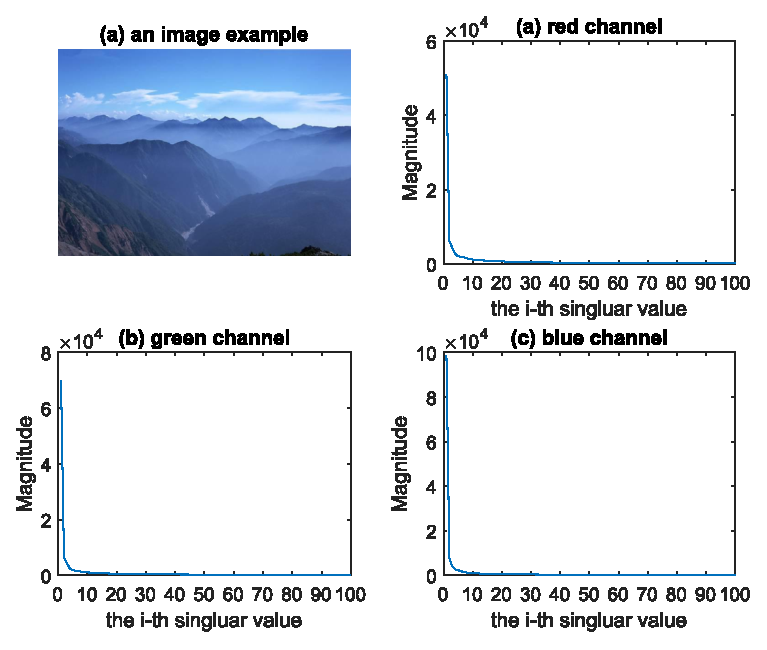
\includegraphics[]{assets/fig1.eps}
	\caption{A 400 $\times$ 500 image example}
	\label{fig1}
\end{figure}

\begin{notations}
	Let $X = (x_1,\cdots, x_n)$ be an m × n matrix, $\Omega \in \{1,\cdots,m\}\times\{1,\cdots,n\}$ denote the indices of the observed
	entries of $X$, and let $\Omega_c$denote the indices of the missing entries. The Forbenius norm of $X$ is defined as $\Vert X \vert_F = \sqrt{\sum_{(i,j)} X^2_{i,j}}$. Let $X=U\Sigma V^T$ be the singular value decomposition for X, where $\Sigma = diag(\sigma_i)$, $1 \leq i\leq \min\{m,n\}$, and $\sigma_i$ is the ith largest singular value of $X$. The nuclear norm of $X$ is denoted as $\Vert X \vert_* = \sum_{i=1}^{\min(m,n)} \sigma_i$ . Let $\mathcal{P}_{\Omega}$ be the orthogonal projection operator onto the span of matrices vanishing outside of  $\Omega$ so that
	\begin{equation*}
		(\mathcal{P}_{\Omega}(X))_{ij} = \begin{cases}
		X_{ij} & \text{\rm if } (i,j) \in \Omega\\
		0 & \text{\rm if } (i,j) \in \Omega^c
	\end{cases}
	\end{equation*}
	The  inner product of the matrix space is defined as $ \langle X,Y\rangle = \sum_{i,j} = X_{ij}Y_{ij}$.
\end{notations}

\begin{definition}
	Consider the SVD of a matrix $X \in \mathbb{R}^{m \times n}$:
	\begin{equation}
		X = U \Sigma V^T, \ \Sigma = diag(\{\sigma_i\}_{1 \leq \min(m,n)}).
	\end{equation}
	Define the singular value shrinkage operator $D_{\tau}$ as follows:
	\begin{equation}
		D_{\tau}(X) = U D_{\tau}(\Sigma) V^T, \ D_{\tau}(\Sigma) = diag(\max\{\sigma_i-\tau,0\}).
	\end{equation}
	We have the following useful theorem:	
\end{definition}

\begin{theorem}
	\label{thm32}
	For each $\tau \geq 0$ and $Y \in \mathbb{R}^{m \times n}$, we have
	\begin{equation}
		D_{\tau}(X) = \underset{X}{\text{\rm arg min}} \frac{1}{2} \Vert X-Y\Vert_F^2 + \tau \Vert X \Vert_*.
	\end{equation} 
\end{theorem}

\section{Related work}
\label{s2}


In this section, we introduce three methods for matrix completion: Optspace, singular value thresholding (SVT) and singular value projection (SVP). These methods are also used to compare with the TNNR algorithm in subsequent experiments. In addition, ADMM and APDL is is briefly explained for better algorithm derivation in Section \ref{s3}.

By approximating the rank function using the nuclear norm to solve the rank
minimization problem \eqref{rmin},  the matrix completion problem can be formulated as follows:
\begin{equation}
	\label{normf}
	\begin{aligned}
		\underset{X}{\text{min}} \ \ \ \ &  \ \ \Vert X\Vert_* \\
		\text{s.t.} \ \ \ \ &  \ \  \mathcal{P}_{\Omega}(X) =  \mathcal{P}_{\Omega}(M),
	\end{aligned}
\end{equation}

For SVT, Cai et al. propose the SVT algorithm :
\begin{equation}
	\begin{aligned}
		\underset{X}{\text{min}} \ \ \ \ &  \ \ \Vert X\Vert_* + \alpha\Vert X\Vert_F^2\\
		\text{s.t.} \ \ \ \ &  \ \  \mathcal{P}_{\Omega}(X) =  \mathcal{P}_{\Omega}(M),
	\end{aligned}
\end{equation}
Construct the Lagrangian function,
\begin{equation}
	\mathcal{L}(X,Y) = \Vert X\Vert_* + \alpha\Vert X\Vert_F^2 + \langle Y, P_{\Omega}(M-X) \rangle,
\end{equation}
where Lagrangian multipliers $Y \in \mathbb{R}^{m \times n}$. SVT solves problem \eqref{normf} using alternating iterative methods,
\begin{equation}
	\begin{aligned}
		X^K & = D_\tau(Y^{k-1})\\
		Y^k & = Y^{k+1} + \sigma_k\mathcal{P}_\Omega(M-X^k).
	\end{aligned}
\end{equation}

For SVP, rewrite \eqref{normf} as:
\begin{equation}
	\begin{aligned}
		\underset{X}{\text{min}} \ \ \ \ &  \ \ \psi (X) = \frac{1}{2}\Vert \mathcal{A}(X) - b\Vert_2^2\\
		\text{s.t.} \ \ \ \ &  \ \  X \in \mathcal{C}(k) = \{X \colon rank(X) \leq k\},
	\end{aligned}
\end{equation}
where $\mathcal{A}$ is affine transformations that satisfy a restricted isometry property.
Construct the Lagrangian function,
\begin{equation}
	\mathcal{L}(X,Y) = \text{min } \Vert \mathcal{A}(X) - b \Vert_F^2.
\end{equation}
The iterative equation is
\begin{equation}
	\begin{aligned}
		Y^{k+1} & = X^{k} - \gamma_k \mathcal{A}^*(\mathcal{A}(X_k)-y)\\
		X^{k+1} & = \text{Trancated SVD}_r(Y_{k+1}).
	\end{aligned}
\end{equation}

For OptSpace, the Lagrangian function of problem \eqref{normf} is
\begin{equation}
	\mathcal{L}(X,Y) = \underset{S \in \mathbb{R}^{r \times r}}{\text{min}} 	\mathcal{L}(X,Y,S) = \frac{1}{2} \Vert \mathcal{P}_\Omega(M-XSY^T)\Vert_F^2+\frac{\lambda}{2}\Vert \mathcal{P}_{\Omega^c}(M-XSY^T)\Vert_F^2
\end{equation}



ADMM algorithm is an important method for solving separable convex optimization problems, with fast processing speed and good convergence performance.The classic ADMM algorithm is suitable for solving the following 2-block (or N-block) convex optimization problems.
\begin{equation}
	\label{admmlg}
	\begin{aligned}
		\underset{x,w}{\text{min}} \ \ \ \ &  \ \ f(x) + g(w)\\
		\text{s.t.} \ \ \ \ &  \ \  Ax+Bw = b,
	\end{aligned}
\end{equation}
where $x \in \mathbb{R}^n$, $w \in \mathbb{R}^m$. And $A \in \mathbb{R}^{p \times n}$, $B \in \mathbb{R}^{p \times m}$, $b \in \mathbb{R}^p$ is convex set.$f$, $g$ is convex function.
Using an augmented Lagrangian with a square regularization term with coefficient $\frac{\beta}{2}$:
\begin{equation}
	\mathcal{L}(x,z,w) = f(x) +g(w) + z^T(Ax+Bw-b) + \frac{\beta}{2} \Vert Ax+Bw-b \Vert_2^2.
\end{equation}
By dual ascent,
\begin{equation}
	\begin{aligned}
		(x^{k+1},w^{k+1}) & \colon = \underset{x,w}{\text{arg min}} \mathcal{L}(x,z^k,w)\\
		z^{k+1} & \colon = z^k + \beta (A x^{k+1} + B w^{k+1} - b).
	\end{aligned}
\end{equation}
Change $(x,w)$ joint optimization to separate alternate iterations and let $y^k = z^k/\beta$,
\begin{equation}
	\begin{aligned}
		x^{k+1} &  = \underset{x}{\text{arg min }} \mathcal{L}_{\beta}(x,y^k,w^{k})\\
		w^{k+1} &  = \underset{w}{\text{arg min }} \mathcal{L}_{\beta}(x^{k+1},y^k,w)\\
		y^{k+1} &  = y^k + (A x^{k+1} + B y^{k+1} - b).
	\end{aligned}
\end{equation}

APGL, also called ast iterative shrinkage-thresholding algorithm (FISTA), solves problems like
\begin{equation}
	\label{apgl}
	\underset{X}{\min} \ g(X)+f(X),
\end{equation}
where $g$ is closed, convex, possibly, nondifferentiable and $f$ is a convex and differentiable function. 
\begin{equation}
	Q(X,Y) = f(Y)+\langle X-Y, \nabla f(Y) \rangle + \frac{1}{2t}\Vert X-Y \Vert_F^2 +g(X).
\end{equation}
Then APGL method solves optimization problem \eqref{apgl} by iteratively updating $X$, $Y$ and $t$. In the $k$-$th$ iteration, we update $X_{k+1}$ as the unique minimizer of $Q(X, Y_k)$:
\begin{equation}
	X_{k+1} = \underset{X}{\text{arg min }}Q(X, Y_k) = \underset{X}{\text{arg min }}g(X)+\frac{1}{2t}\Vert X- (Y_k -t_k \nabla f(Y_k))\Vert_F^2.
\end{equation}


\section{Truncated nuclear norm regularization}
\label{s3}

\subsection{The approach proposed by Yao Hu et al.}
By using Truncated nuclear norm, this approach achieves a better approximation of the rank function than the nuclear norm.
\begin{definition}
	Given a matrix $X \in \mathbb{R}^{m \times n}$, the truncated nuclear norm $\Vert X \vert_r$ is defined as the sum of min$(m,n) - r$  minimum singular values, i.e., $\Vert X \vert_r = \sum_{i=r+1}^{\min(m,n)} \sigma_i(X)$ .
\end{definition}

Thus, the objective function of this approach can be formulated as follows
\begin{equation}
	\label{obj0}
	\begin{aligned}
		\underset{X}{\text{min}} \ \ \ \ &  \ \ \Vert X\Vert_r \\
		\text{s.t.} \ \ \ \ &  \ \  \mathcal{P}_{\Omega}(X) =  \mathcal{P}_{\Omega}(M).
	\end{aligned}
\end{equation}
Since $\Vert X\Vert_r$ is non-convex, they propose the follow theorem:
\begin{theorem}
	\label{thm31}
	For any given matrix $X \in \mathbb{R}^{m \times n}$, any matrices $A \in \mathbb{R}^{r \times m}$, $B \in \mathbb{R}^{r \times m}$ that $AA^T = I_{r \times r}$. For any nonnegative integer $r \ (r \leq \min(m,n))$, we have 
	\begin{equation}
		\label{eq31}
		\text{\rm Tr}(AXB^T) \leq \sum_{i=1}^r \sigma_i(X).
	\end{equation}
\end{theorem}
The proof is given in the Appendix.

Suppose, $U\Sigma V^T$ is the singular value decomposition of $X$, where $U = (\bm u_1,\dots,\bm u_m) \in \mathbb{R}^{m \times m}$, $\Sigma \in \mathbb{R}^{m \times n}$, and $V = (\bm v_1,\dots,\bm v_m) \in \mathbb{R}^{n \times n}$. The equality of holds when 
\begin{equation}
	\label{}
	A = (\bm u_1,\dots,\bm u_m)^T, \ B = (\bm v_1,\dots,\bm v_m)^T.
\end{equation}
This is because
\begin{equation}
	\begin{aligned}
		\label{treq}
		\text{Tr} ((\bm u_1,\dots,\bm u_m)^TX(\bm v_1,\dots,\bm v_m))
		& = \text{Tr} ((\bm u_1,\dots,\bm u_m)^TU\Sigma V^T(\bm v_1,\dots,\bm v_m)) \\
		& = \text{Tr} (((\bm u_1,\dots,\bm u_m)^TU) \Sigma (V^T(\bm v_1,\dots,\bm v_m))) \\
		& = \text{Tr} \left( \begin{bmatrix}
			I_r & 0\\
			0 & 0 
		\end{bmatrix} \Sigma \begin{bmatrix}
			I_r & 0\\
			0 & 0 
		\end{bmatrix}
		\right) \\
		& = \text{Tr}(diag(\sigma_1(X),\dots,\sigma_r(X),0,\dots,0)) \\
		& = \sum_{i=1}^r \sigma_i(X)	
	\end{aligned}
\end{equation}
Combining \eqref{eq31} and \eqref{treq}, we get
\begin{equation}
	\underset{AA^T=I,BB^T=I}{max} \text{Tr}(AXB^T) \leq \sum_{i=1}^r \sigma_i(X).
\end{equation}
Then we have 
\begin{equation}
	\Vert X\Vert_* - \underset{AA^T=I,BB^T=I}{max} \text{Tr}(AXB^T)  
		= \sum_{i=1}^{\min(m,n)} \sigma_i(X) - \sum_{i=1}^r \sigma_i(X) 
		= \Vert X\Vert_r
\end{equation}
Thus, the optimization problem \eqref{obj0} can be rewritten as follows:
\begin{equation}
\begin{aligned}
	\label{obj1}
	\underset{X}{\text{min}} \ \ \ \ &  \ \  \Vert X\Vert_* - \underset{AA^T=I,BB^T=I}{max} \text{Tr}(AXB^T) \\
	\text{s.t.} \ \ \ \ &  \ \  \mathcal{P}_{\Omega}(X) =  \mathcal{P}_{\Omega}(M),
\end{aligned}
\end{equation}
where $A \in \mathbb{R}^{r \times m}$, $B \in \mathbb{R}^{r \times m}$.

Based on \eqref{obj1},  they design a simple but efficient iterative scheme, which is summarized in Algorithm \ref{algo1}. In the $l$th iteration, we first fix $X_l$ and compute $A_l$ and $B_l$ . And then we fix $A_l$ and $B_l$ ro update $X_{l+1}$ by  solving the following problem:
\begin{equation}
	\label{obj2}
\begin{aligned}
	\underset{X}{\min} \ \ \ \ & \ \  \Vert X \Vert_* - \text{Tr}(AXB^T) \\
	\text{s.t.} \ \ \ \ & \ \    \mathcal{P}_{\Omega}(X) =  \mathcal{P}_{\Omega}(M).
\end{aligned}
\end{equation}

\begin{algorithm}[t]
	\caption{The Proposed Two-Step Approach for Sovling (6)}
	\label{algo1}
	\textbf{Input:} original incomplete data matrix $M_{\Omega}$, where $\Omega$ is the indices of the observed entries, tolerance $\epsilon_0$ \\
	\textbf{Initialization:} $X_1 = \mathcal{P}_{\Omega}(M)$. 
	\begin{algorithmic}
		\Repeat 
		\State \textbf{step 1.} Given $X_l$, compute $U_l, \Sigma_l, V_l = svd(X_l)$, 
		\State where $U_l = (\bm u_1,\dots,\bm u_m) \in \mathbb{R}^{m \times m}$, $V_l = (\bm v_1,\dots,\bm v_m) \in \mathbb{R}^{n \times n}$. 
		\State Compute $A_l$ and $B_l$, as $A_l = (\bm u_1,\dots,\bm u_m)^T, \ B_l = (\bm v_1,\dots,\bm v_m)^T$
		\State \textbf{step 2.} Solve $X_{l+1} = \underset{X}{\text{arg min}} \Vert X \Vert_* - \text{Tr}(AXB^T) \qquad \text{s.t.} \quad \mathcal{P}_{\Omega}(X) =  \mathcal{P}_{\Omega}(M)$ 
		\Until{$\Vert X_{l+1} - X_l \Vert_F \leq \epsilon_0$.}
		\State \Return the recovered matrix.
	\end{algorithmic}
\end{algorithm}



\subsection{The optimization using TNNR-ADMM}
ADMM is a method for solving a decomposable convex optimization problem. It can equivalently decompose the objective function of the original problem into several solvable sub-problems, then solve each sub-problem in parallel, and finally coordinate the solutions of the sub-problems to obtain the global solution of the original problem.

By using ADMM to solve \eqref{obj2}, an optimization algorithm TNNR-ADMM is proposed. First, rewrite \eqref{obj2} as follows:
\begin{equation}
	\label{objadmm}
	\begin{aligned}
		\underset{X,W}{\min} \ \ \ \ & \ \  \Vert X \Vert_* - \text{Tr}(A_l X B_l^T) \\
		\text{s.t.} \ \ \ \ & \ \    X=W, \ \mathcal{P}_{\Omega}(X) =  \mathcal{P}_{\Omega}(M).
	\end{aligned}
\end{equation}
By \eqref{admmlg}, we have $f(X)=\Vert X \Vert_*$ and $g(W) = \text{Tr}(A_l X B_l^T)$. 

The augmented lagrange function of is 
\begin{equation}
	L(X,Y,W,\beta) = \Vert X \Vert_* - \text{Tr}(A_l X B_l^T) + \frac{\beta}{2}\Vert X-W \Vert_F^2 + Tr(Y^T(X-W)),
\end{equation}
where $\beta > 0$ is  the penalty parameter. Given the initial setting $X_1 = \mathcal{P}_\Omega(M)$, $W_1 = X_1$, and $Y_1 =  X_1$, the optimization problem \eqref{objadmm} can be solved via the following three steps.

$\textit{Computing}$  $X_{k+1}$. Fix $W_k$ and $Y_k$, and minimize $L(X,Y_k,W_k,\beta)$ for $X_{k+1}$ as follows:
\begin{equation}
\begin{aligned}
	X_{k+1} & =\underset{X}{\text{arg min}}\ L(X,Y_k,W_k,\beta) \\
	& =  \underset{X}{\text{arg min}} \ \Vert X\Vert_* - Tr(A_l W_k B_l^T)    + \frac{\beta}{2}\Vert X-W_k \Vert_F^2 + Tr(Y_k^T(X-W_k))
\end{aligned}
\end{equation}
Ignoring constant terms, this can be rewritten as 

\begin{equation}
	X_{k+1} = \underset{X}{\text{arg min}} \ \Vert X\Vert_* + \frac{\beta}{2} \Vert X-\left(W_k - \frac{1}{\beta}Y_k \right) \Vert_F^2
\end{equation}


By Theorem~\ref{thm32} ,we can solve the above problem as
\begin{equation}
	\label{admmx}
X_{k+1} = D_{\frac{1}{\rho}}(W_k - \frac{1}{\rho}Y_k).
\end{equation}


$\textit{Computing}$  $W_{k+1}$. Fix $X_{k+1}$ and $Y_k$ to calculate $W_{k+1}$ as follows:
\begin{equation}
\begin{aligned}
	W_{k+1}& = \underset{\mathcal{P}_{\Omega}(W) = \mathcal{P}_{\Omega}(M)}{\text{arg min}} \ L(X_{k+1},Y_k,W,\beta) \\
	& =  \underset{\mathcal{P}_{\Omega}(W) = \mathcal{P}_{\Omega}(M)}{\text{arg min}} \ \Vert X_{k+1}\Vert_* - Tr(A_l W B_l^T)    + \frac{\beta}{2}\Vert X_{k+1}-W \Vert_F^2 + Tr(Y_k^T(X_{k+1}-W)).
\end{aligned}
\end{equation}
then we get
\begin{equation}
	W_{k+1} = X_{k+1} + \frac{1}{\beta}(A_l^TB_l + Y_k).
\end{equation}

fix the values at the observed entries
\begin{equation}
	W_{k+1} = \mathcal{P}_{\Omega^c}(X_{k+1}) + \mathcal{P}_{\Omega}(M).
\end{equation}

$\textit{Computing}$  $Y_{k+1}$. Fix $X_{k+1}$ and $W_{k+1}$ to calculate $Y_{k+1}$ as follows:
\begin{equation}
	Y_{k+1} = Y_{k} + \beta(X_{k+1} - W_{k+1}).
\end{equation}

The whole procedure of TNNR-ADMM is summarized in Algorithm \ref{algo2}.


\begin{algorithm}[t]
	\caption{The Optimization using TNNR-ADMM}
	\label{algo2}
	\textbf{Input:} $A_l$, $B_l$, $M_{\Omega}$, and tolerance $\epsilon$ are given.\\
	\textbf{Initialization:} $X_1 = M_{\Omega}$, $W_1 = X_1$, $Y_1=X_1$, and $\beta = 1$. 
	\begin{algorithmic}
		\Repeat 
		\State \textbf{step 1.} $X_{k+1} = D_{\frac{1}{\rho}}(W_k - \frac{1}{\rho}Y_k)$.
		\State \textbf{step 2.} $W_{k+1} = X_{k+1} + \frac{1}{\beta}(A_l^TB_l + Y_k)$.
		\State Fix values at observed entries, 
		$W_{k+1} = X_{k+1} + \frac{1}{\beta}(A_l^TB_l + Y_k)$.
		\State \textbf{step 3.} $Y_{k+1} = Y_{k} + \beta(X_{k+1} - W_{k+1})$.
		\Until{$\Vert X_{k+1} - X_k \Vert_F \leq \epsilon$.}
	\end{algorithmic}
\end{algorithm}

\subsection{The optimization using TNNR-APGL}
Considering the noisy data in the real applications, it is beneficial to relax the constrained problem \eqref{obj2} into
\begin{equation}
	\label{apglobj}
	\min \Vert X\Vert_* - \text{Tr}(A_lXB_l^T) + \frac{\lambda}{2}\Vert X_\Omega - M_\Omega \Vert^2_F,
\end{equation}
for some $\lambda >0$.

According to \eqref{apgl}, in problem \eqref{apglobj}, we choose
\begin{equation*}
	g(x) = \Vert X\Vert_*,
\end{equation*}
and
\begin{equation*}
	f(x) = - \text{Tr}(A_lXB_l^T) + \frac{\lambda}{2}\Vert X_\Omega - M_\Omega \Vert^2_F.
\end{equation*}

By Theorem~\ref{thm32}, we get
\begin{equation}
	\begin{aligned}
		X_{k+1} & = \underset{X}{\text{arg min }} \Vert X\Vert_* + \frac{1}{2t}\Vert X- (Y_k -t_k \nabla f(Y_k))\Vert_F^2 \\
		& = \mathcal{D}_{t_k}(Y_k - t_k\nabla f(Y_k)) \\
		& = \mathcal{D}_{t_k}(Y_k - t_k(A_l^TB_l - \lambda(\mathcal{P}_{\Omega}(Y_k)- \mathcal{P}_{\Omega}(M)))).
	\end{aligned}
\end{equation}

Finally, $t_{k+1}$ and $Y_{k+1}$ are updated as:
\begin{equation}
	\begin{aligned}
		t_{k+1} & = \frac{1+\sqrt{1+4t^2_k}}{2}, \\
		Y_{k+1}& = X_{k+1} +\frac{t_{k}-1}{t_{k+1}}(X_{k+1}-X_{k}). \\
	\end{aligned}
\end{equation}

The procedures of solving (26) are summarized in Algorithm \ref{algo3}.

\begin{algorithm}[t]
	\caption{The Optimization using TNNR-APGL}
	\label{algo3}
	\textbf{Input:} $A_l$, $B_l$, $M_{\Omega}$, and tolerance $\epsilon$ are given.\\
	\textbf{Initialization:} $t_1 = 1$, $X_1 = M_{\Omega}$, $Y_1=X_1$.
	\begin{algorithmic}
		\Repeat 
		\State \textbf{step 1.} $X_{k+1} = \mathcal{D}_{t_k}(Y_k - t_k(A_l^TB_l - \lambda(\mathcal{P}_{\Omega}(Y_k)- \mathcal{P}_{\Omega}(M))))$.
		\State \textbf{step 2.} $t_{k+1} = \frac{1+\sqrt{1+4t^2_k}}{2}$.
		\State \textbf{step 3.} $Y_{k+1} = X_{k+1} +\frac{t_{k}-1}{t_{k+1}}(X_{k+1}-X_{k})$.
		\Until{$\Vert X_{k+1} - X_k \Vert_F \leq \epsilon$.}
	\end{algorithmic}
\end{algorithm}


\subsection{The optimization using TNNR-ADMMAP}
In Algorithm 2, the two constraints are considered separately, but the inconsistency of the two constraints may slow down the convergence.
By combining the two constraints into a new constraint in a special way and adding an adaptive penalty parameter to speed up the convergence,  a new approach by using the ADMM with adaptive penalty (TNNR-ADMMAP) is proposed.
\subsubsection{The reformulation of problem }
To deal with the two constraints simultaneously, in this section, we reformulate the problem \ref{objadmm} as follows:
\begin{equation}
	\label{apobj}
	\begin{aligned}
		\underset{X}{\min} \ \ \ \ & \ \  \Vert X \Vert_* - \text{Tr}(A_lXB_l^T) \\
		\text{s.t.} \ \ \ \ & \ \    \mathcal{A}(X) + \mathcal{B}(M) = \mathcal{C},
	\end{aligned}
\end{equation}
where $\mathcal{A}$ and $\mathcal{B}$ : $\mathbb{R}^{m\times n} \rightarrow \mathbb{R}^{2m\times 2n}$ are linear opertors defined as follows:
\begin{equation*}
	\mathcal{A}(X) = \begin{pmatrix}
		X & 0 \\
		0 & 0
	\end{pmatrix}, \
	\mathcal{B}(X) = \begin{pmatrix}
		-W & 0 \\
		0 & \mathcal{P}_\Omega(X)
	\end{pmatrix}, \ 
	\mathcal{C} = \begin{pmatrix}
		0 & 0 \\
		0 & \mathcal{P}_\Omega(M)
	\end{pmatrix}.
\end{equation*}
Then discuss the properties of adjoint operators $\mathcal{A}$ and $\mathcal{B}$.

Suppose
\begin{equation*}
	Y = \begin{pmatrix}
		Y_{11} & Y_{12} \\
		Y_{21} & Y_{22}
	\end{pmatrix},
\end{equation*}
where $Y_{ij} \in \mathbb{R}^{m \times n}$, $i=1,2$ and $j=1,2$. Denote $\mathcal{A}^*$, $\mathcal{B}^*$ : $\mathbb{R}^{2m \times 2n} \rightarrow \mathbb{R^{m \times n}} $ as the adjoint operators of $\mathcal{A}$ and $\mathcal{B}$ separately satisfying 
\begin{equation}
	\label{adjopt}
	\langle \mathcal{A}(X),Y \rangle = \langle X,\mathcal{A}^*(Y) \rangle,\ \langle \mathcal{B}(X),Y \rangle =  \langle X,\mathcal{B}^*(Y)
\end{equation}
By the definition of operators $\mathcal{A}$ and $\mathcal{B}$, it is easy to verify that
\begin{equation*}
	\langle \mathcal{A}(X),Y \rangle = \text{Tr}\begin{pmatrix}
		X & 0 \\
		0 & 0 
	\end{pmatrix}\begin{pmatrix}
		Y_{11} & Y_{12} \\
		Y_{21} & Y_{22}
	\end{pmatrix}^T = \text{Tr}(XY_{11}^T) = \langle X,Y_{11} \rangle
\end{equation*}
and 
\begin{equation*}
	\begin{aligned}
		\langle \mathcal{B}(W),Y \rangle & = \text{Tr}\begin{pmatrix}
			-W & 0 \\
			0 & \mathcal{P}_\Omega(W) 
		\end{pmatrix}\begin{pmatrix}
			Y_{11} & Y_{12} \\
			Y_{21} & Y_{22}
		\end{pmatrix}^T \\
		& = \text{Tr}\begin{pmatrix}
			-WY_{11}^T & -WY_{21}^T \\
			\mathcal{P}_\Omega(W)Y_{11}^T & \mathcal{P}_\Omega(W)Y_{22}^T
		\end{pmatrix}\\
		&= \langle W, -Y_{11} \rangle + \langle W, \mathcal{P}_\Omega(Y_{22}) \rangle \\
		& = \langle W, -Y_{11}+ \mathcal{P}_\Omega(Y_{22})  \rangle.
	\end{aligned}
\end{equation*}

By the definition of the adjoint operator \eqref{adjopt}, the adjoint operators  $\mathcal{A}$ and $\mathcal{B}$ can be computed as 
\begin{equation}
	\label{optab}
	\begin{aligned}
		\mathcal{A}^*(Y) & = Y_{11}, \\
		\mathcal{B}^*(Y) & = -Y_{11} + \mathcal{P}_\Omega(Y_{22}).
	\end{aligned}
\end{equation}

Let us rewrite the augmented Lagrange function for the optimization problem \eqref{apobj} as 
\begin{equation}
\mathcal{L}_{AP}(X,W,Y,\beta) = -\text{Tr}(A_lWB_l^T) + \langle Y, \mathcal{A}(X)+\mathcal{B}(W) -\mathcal{C} \rangle + \Vert X\Vert_* + \frac{\beta}{2}\Vert \mathcal{A}(X)+\mathcal{B}(W) -\mathcal{C} \Vert^2_F,
\end{equation}
where $Y$ is the Lagrange multiplier matrix and $\beta >0$ is the penalty parameter. The iterative scheme of ADMM for problem \eqref{apobj} is given as follows:
	\begin{align}
		\label{apx}
		X_{k+1} & = \underset{X}{\text{arg min }} \mathcal{L}_{AP}(X,W_k,Y_k,\beta) \nonumber\\
		& = \underset{X}{\text{arg min }}\frac{\beta}{2}\Vert \mathcal{A}(X) + \mathcal{B}(W_k) - \mathcal{C} + \frac{1}{\beta}Y_{k} \Vert_F^2 + \Vert X \Vert_*,
	\end{align}
	\begin{align}
		\label{apw}
		W_{k+1} & = \underset{W}{\text{arg min }} \mathcal{L}_{AP}(X_{k+1},W,Y_k,\beta)  \nonumber \\
		& = \underset{W}{\text{arg min }}\frac{\beta}{2}\Vert \mathcal{A}(X_{k+1}) + \mathcal{B}(W) - \mathcal{C} + \frac{1}{\beta}Y_{k} \Vert_F^2 -\text{Tr}(A_lWB_l^T),
	\end{align}

\begin{equation}
	\label{apy}
	Y_{k+1} = Y_{k}+\beta[\mathcal{A}(X_{k+1})+\mathcal{B}(W)-\mathcal{C}].
\end{equation}

%\begin{equation}
%	\label{apx}
%	\begin{aligned}
%		X_{k+1} & = \underset{X}{\text{arg min }} \mathcal{L}_{AP}(X,W_k,Y_k,\beta) \\
%		& = \underset{X}{\text{arg min }}\frac{\beta}{2}\Vert \mathcal{A}(X) + \mathcal{B}(W_k) - \mathcal{C} + \frac{1}{\beta}Y_{k} \Vert_F^2 + \Vert X \Vert_* , \\
%		W_{k+1} & = \underset{W}{\text{arg min }} \mathcal{L}_{AP}(X_{k+1},W,Y_k,\beta) \\
%		& = \underset{W}{\text{arg min }}\frac{\beta}{2}\Vert \mathcal{A}(X_{k+1}) + \mathcal{B}(W) - \mathcal{C} + \frac{1}{\beta}Y_{k} \Vert_F^2 -\text{Tr}(A_lWB_l^T), \\
%	Y_{k+1} & = Y_{k}+\beta[\mathcal{A}(X_{k+1})+\mathcal{B}(W)-\mathcal{C}].
%		\end{aligned}
%\end{equation}

\subsubsection{The iterative scheme of TNNR-ADMMAP}
Based on the iterative scheme \eqref{apx}-\eqref{apy}, TNNR-ADMMAP algorithm is introduced.

$\textit{Computing}$  $X_{k+1}$.
\begin{equation}
	\begin{aligned}
			X_{k+1} & = \underset{X}{\text{arg min }}\frac{\beta}{2}\Vert \mathcal{A}(X) + \mathcal{B}(W_k) - \mathcal{C} + \frac{1}{\beta}Y_{k} \Vert_F^2 + \Vert X \Vert_* \\
			& = \underset{X}{\text{arg min }}\frac{\beta}{2}\Vert P \Vert^2_F + \Vert X\Vert_*,
	\end{aligned}
\end{equation}
where 
\begin{equation*}
	P = \begin{pmatrix}
		X- W_k + \frac{1}{\beta} & \frac{1}{\beta} (Y_k)_{12} \\
		\frac{1}{\beta}(Y_k)_{21} & \mathcal{P}_\Omega + \frac{1}{\beta}(Y_k)_{22}
	\end{pmatrix}.
\end{equation*}
By Theorem \eqref{thm32}, we get
\begin{equation}
	X_{k+1} = \mathcal{D}\left(W_k - \frac{1}{\beta}(Y_k)_{11}\right).
\end{equation}

$\textit{Computing}$  $W_{k+1}$. Setting the first derivative of
$\mathcal{L}_{AP}(X_{k+1},W,Y_k,\beta)$ to zero, we get
\begin{equation*}
	\beta \mathcal{B}^*\left[ \mathcal{B}(W) + \mathcal{A} (X_{k+1} ) - \mathcal{C} +\frac{1}{\beta} Y_k \right] - A_l^TB_l = 0,
\end{equation*}
which can be rewritten as
\begin{equation}
	\mathcal{B}^*\mathcal{B}(W) = \frac{1}{\beta}A_l^TB_l - \mathcal{B}^*\left[ \mathcal{A} (X_{k+1} ) - \mathcal{C} +\frac{1}{\beta} Y_k \right].
\end{equation}

From the property of adjoint operator $\mathcal{B}^*$, the left-hand side of the above equation can be rewritten as
\begin{equation}
	\label{w1}
	\mathcal{B}^*\mathcal{B}(W) = \mathcal{B}^* \begin{pmatrix}
		-W & 0 \\
		0 & \mathcal{P}_\Omega(W)
	\end{pmatrix} = W + \mathcal{P}_\Omega(W).
\end{equation}

Then we apply the orthogonal projection operator $\mathcal{P}_\Omega$ on both sides of \eqref{w1}, and finally we get
\begin{equation}
	\label{w2}
	\mathcal{P}_\Omega(W) = \frac{1}{2} \mathcal{P}_\Omega(\mathcal{B}^*\mathcal{B}(W)).
\end{equation}
From \eqref{w1} and \eqref{w2}, we obtain
\begin{equation*}
	W_{k+1} = \mathcal{B}^*\mathcal{B}(W) - \mathcal{P}_\Omega(W) = \mathcal{B}^*\mathcal{B}(W) -\frac{1}{2} \mathcal{P}_\Omega(\mathcal{B}^*\mathcal{B}(W)). 
\end{equation*}

Then compute $	\mathcal{B}^*\mathcal{B}(W)$ directly as follows:
\begin{align*}
	\mathcal{B}^*\mathcal{B}(W) &=  \frac{1}{\beta}A_l^TB_l - \mathcal{B}^*\left[ \mathcal{A} (X_{k+1} ) - \mathcal{C} +\frac{1}{\beta} Y_k \right] \\
	& = \frac{1}{\beta}A_l^TB_l - \mathcal{B}^*\left[\begin{pmatrix}
		X_{k+1} & 0 \\
		0 & 0
	\end{pmatrix} - 
	\begin{pmatrix}
		0 & 0 \\
		0 & \mathcal{P}_\Omega
	\end{pmatrix} + \frac{1}{\beta} 
	\begin{pmatrix}
		(Y_k)_{11} & (Y_k)_{12} \\
		(Y_k)_{21} & (Y_k)_{22}
	\end{pmatrix}\right] \\
	& = -\mathcal{B}^*\begin{pmatrix}
		\frac{1}{\beta} (Y_k)_{11} + X_{k+1} & \frac{1}{\beta} (Y_k)_{12} \\
		\frac{1}{\beta} (Y_k)_{21} & \frac{1}{\beta} (Y_k)_{22} - \mathcal{P}_\Omega(M)
	\end{pmatrix} + \frac{1}{\beta}A_l^TB_l
\end{align*}

From property \eqref{optab} of the adjoint operator $\mathcal{B}^*$, we can get 
\begin{equation*}
	\mathcal{B}^* \begin{pmatrix}
				\frac{1}{\beta} (Y_k)_{11} + X_{k+1} & \frac{1}{\beta} (Y_k)_{12} \\
		\frac{1}{\beta} (Y_k)_{21} & \frac{1}{\beta} (Y_k)_{22} - \mathcal{P}_\Omega(M)
	\end{pmatrix} = -\left(\frac{1}{\beta}(Y_k)_{11} + X_{k+1} \right) + \mathcal{P}_\Omega(\frac{1}{\beta} (Y_k)_{22}-M).
\end{equation*}
Thus,
\begin{equation}
	\label{w3}
	\mathcal{B}^*\mathcal{B}(W) = - \left[-\left(\frac{1}{\beta}(Y_k)_{11} + X_{k+1} \right) + \mathcal{P}_\Omega(\frac{1}{\beta} (Y_k)_{22}-M) \right] + \frac{1}{\beta}A_l^TB_l.
\end{equation}
Based on \eqref{w2} and \eqref{w3}, we obtain
\begin{equation}
	W_{k+1} = \frac{1}{2\beta} \mathcal{P}_\Omega [\beta(M-X_{k+1}) - (A_l^TB_l + (Y_k)_{11}+ (Y_k)_{22})] + X_{k+1} +  \frac{1}{\beta}(A_l^TB_l + (Y_k)_{11}).
\end{equation}

$\textit{Computing}$  $Y_{k+1}$. The update of Lagrange multipliers is the same as \eqref{apy}.

\subsubsection{Adapive penalty}
For a fixed penalty parameter, if it is chosen to be too small or too large, the computational cost will increase significantly. At the same time, finding the optimal penalty parameter is difficult. Therefore, dynamic adjustment of penalty parameters may be better in practical applications. The adaptive update strategy adopted is as follows:
\begin{equation}
	\label{beta1}
	\beta_{k+1} = \min(\beta_{max}, \rho \beta_k),
\end{equation}
where $\beta_{max}$ is an upper bound of $\beta_k$. The value of $\rho$ is defined as
\begin{equation}
	\label{beta2}
	\rho = \left\{
		\begin{aligned}
			\rho_0, \quad & \text{if} \; \frac{\beta_k \max\{ \Vert X_{k+1} - X_k \Vert_F \}}{ \Vert \mathcal{C} \Vert_F} < \kappa \\
			1, \quad & \text{otherwise},
		\end{aligned}
	\right.
\end{equation}
where $\rho > 1$ is a constant and $\kappa >0 $ is a threshold chosen in advance. When the difference between $(X_{k+1}, W_{k+1})$ and $(X_{k}, W_{k})$ is small enough, $\beta_{k+1}$ increases to $\rho_0\beta_k$ and the convergence rate is improved.

The procedures of TNNR-ADMMAP are summarized in Algorithm \ref{algo4}.

\begin{algorithm}[t]
	\caption{Inner Optimization by ADMMAP}
	\label{algo4}
	\textbf{Input:} $A_l$, $B_l$, $M_{\Omega}$, and tolerance $\epsilon$ are given.\\
	\textbf{Initialization:} $t_1 = 1$, $X_1 = M_{\Omega}$, $Y_1=X_1$.
	\begin{algorithmic}
		\Repeat 
		\State \textbf{step 1.} $X_{k+1} = \mathcal{D}\left(W_k - \frac{1}{\beta}(Y_k)_{11}\right)$.
		\State \textbf{step 2.} $W_{k+1} = \frac{1}{2\beta} \mathcal{P}_\Omega [\beta(M-X_{k+1}) - (A_l^TB_l + (Y_k)_{11}+ (Y_k)_{22})]$ \\
		$ \quad\quad\quad\quad\quad\quad\quad\quad+ X_{k+1} +  \frac{1}{\beta}(A_l^TB_l + (Y_k)_{11})$.
		\State \textbf{step 3.} $Y_{k+1} = Y_{k}+\beta[\mathcal{A}(X_{k+1})+\mathcal{B}(W)-\mathcal{C}]$.
		\State \textbf{step 4.} Update $\beta_k$ by \eqref{beta1} and \eqref{beta2}
		\Until{$\Vert X_{k+1} - X_k \Vert_F \leq \epsilon$.}
	\end{algorithmic}
\end{algorithm}



\section{Experimental results}
\label{s4}

In this section, we conduct experiments on synthetic data and real visual data, and compare six matrix completion algorithms: SVT, SVP, OptSapce, TNNR-ADMM, TNNR-APGL, and TNNR-ADMMAP.

\subsection{Synthetic data}
We generate $m \times n$ matrices of rank $r_0$ by sampling two matrices, i.e., $M_L \in \mathbb{R}^{m \times r_0} $ and $M_R \in \mathbb{R}^{r_0 \times m} $, each having i.i.d. Gaussian entries, and setting $M=M_l M_R$. The localtions of observed indices $\Omega$ are sampled uniformly at random. Let $p$ be the  percentage of observed entries over $m \times n$. We generate synthetic data as follows:
\begin{equation*}
	B = M+ \sigma Z, \ B_{ij} = M_{ij} + \sigma Z_{ij}, \ (i,j) \in \Omega,
\end{equation*}
where $Z \sim \mathcal{N} (0,1)$. Denote the full noiseless matrix as $X_{full}$ and the solution given by an algorithm as $X_{sol}$, define a commonly used criterion in matrix completion:
\begin{equation*}
	\text{total reconstruction error} = \Vert \mathcal{P}_{\Omega^c}(X_{sol}-X_{full})\Vert_F.
\end{equation*}

Denote different matrix ranks as $r_0$ and differnet nosie levels as $\sigma$.
We compare the reconstruction error of the six methods under different setting:
\begin{itemize}
	\item  the matrix size $m =100$, $n=200$, $r_0 = 10$. Fig.~\ref{fig2} shows the results under different noise levels and different observed ratios.
	\item  the matrix size $m =100$, $n=200$, $\sigma = 0.5$. Fig.~\ref{fig3} shows the results under different ranks and different observed ratios.
\end{itemize}

\begin{figure}[htbp]
	\label{fig2ori}
	\centering
	\subfloat[$60 \%$ observed]{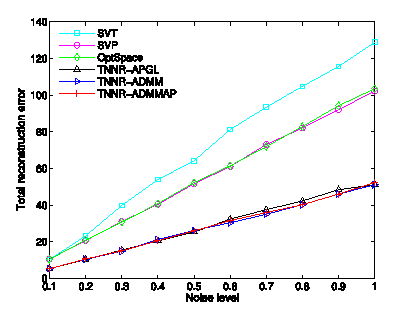
\includegraphics[width=0.45\textwidth]{./assets/ori-fig2-60.eps}}\quad\quad
	\subfloat[$70 \%$ observed]{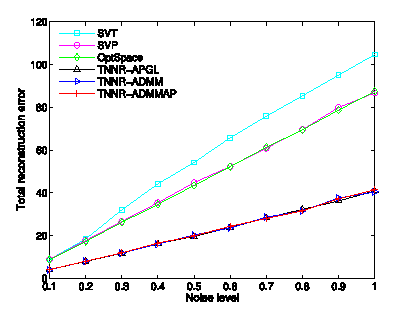
\includegraphics[width=0.45\textwidth]{./assets/ori-fig2-70.eps}}\\
	\subfloat[$80 \%$ observed]{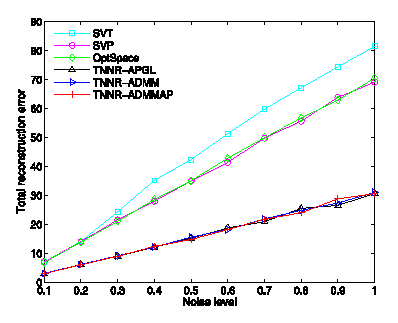
\includegraphics[width=0.45\textwidth]{./assets/ori-fig2-80.eps}}\quad\quad
	\subfloat[$90 \%$ observed]{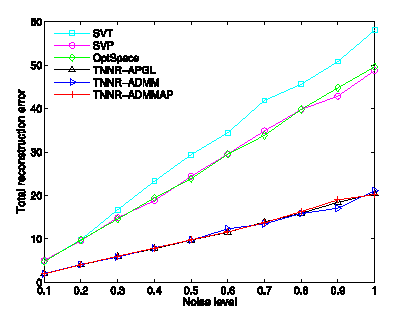
\includegraphics[width=0.45\textwidth]{./assets/ori-fig2-90.eps}}\\
	\caption{ The reconstruction error versus the noise level using the synthetic dataset. (The original result of paper)}
\end{figure}
\begin{figure}[htbp]
	\label{fig2}
	\centering
	\subfloat[$60 \%$ observed]{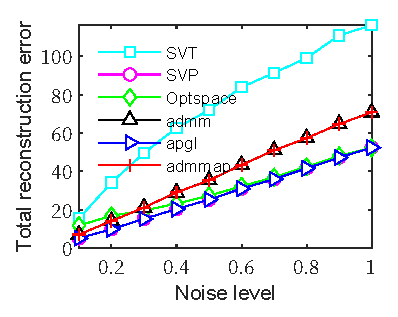
\includegraphics[width=0.45\textwidth]{./assets/fig2-60.eps}}\quad\quad
	\subfloat[$70 \%$ observed]{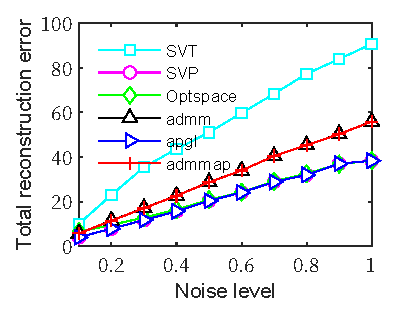
\includegraphics[width=0.45\textwidth]{./assets/fig2-70.eps}}\\
	\subfloat[$80 \%$ observed]{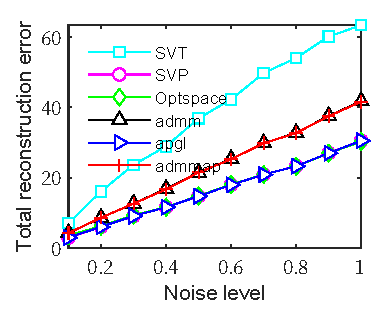
\includegraphics[width=0.45\textwidth]{./assets/fig2-80.eps}}\quad\quad
	\subfloat[$90 \%$ observed]{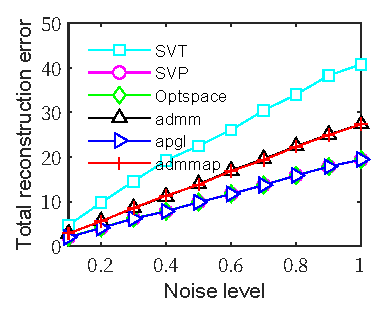
\includegraphics[width=0.45\textwidth]{./assets/fig2-90.eps}}\\
	\caption{ The reconstruction error versus the noise level using the synthetic dataset. (The results we reproduced)}
\end{figure}

\begin{figure}[htbp]
	\label{fig3ori}
	\centering
	\subfloat[$60 \%$ observed]{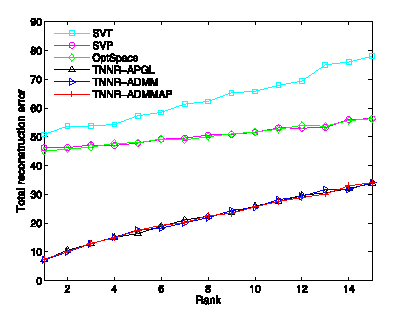
\includegraphics[width=0.45\textwidth]{./assets/ori-fig3-60.eps}}\quad\quad
	\subfloat[$70 \%$ observed]{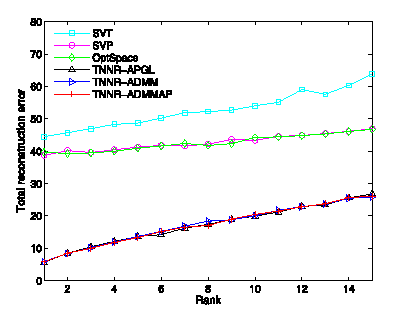
\includegraphics[width=0.45\textwidth]{./assets/ori-fig3-70.eps}}\\
	\subfloat[$80 \%$ observed]{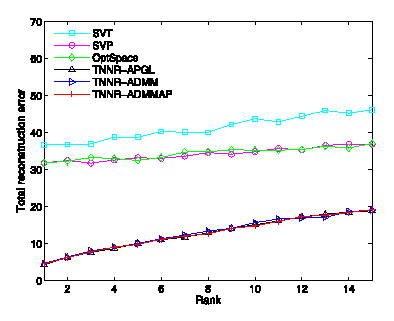
\includegraphics[width=0.45\textwidth]{./assets/ori-fig3-80.eps}}\quad\quad
	\subfloat[$90 \%$ observed]{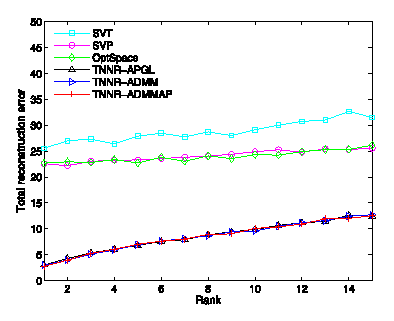
\includegraphics[width=0.45\textwidth]{./assets/ori-fig3-90.eps}}\\
	\caption{Recovery of an incomplete image with random mask. (The original result of paper)}
\end{figure}
\begin{figure}[htbp]
	\label{fig3}
	\centering
	\subfloat[$60 \%$ observed]{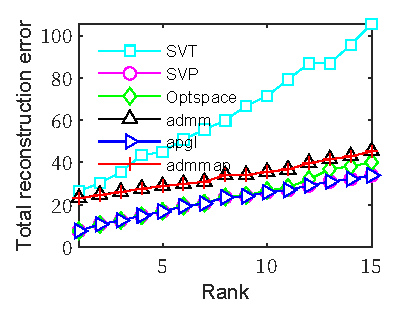
\includegraphics[width=0.45\textwidth]{./assets/fig3-60.eps}}\quad\quad
	\subfloat[$70 \%$ observed]{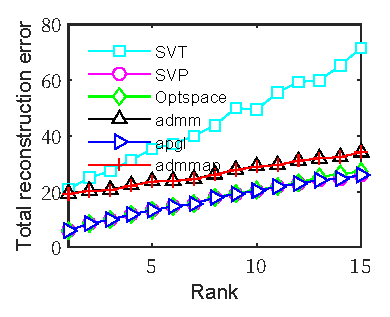
\includegraphics[width=0.45\textwidth]{./assets/fig3-70.eps}}\\
	\subfloat[$80 \%$ observed]{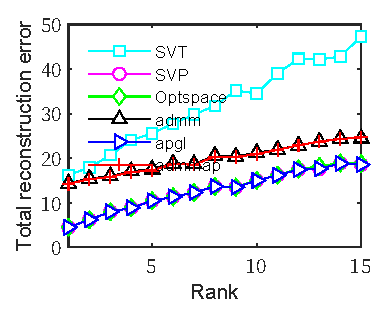
\includegraphics[width=0.45\textwidth]{./assets/fig3-80.eps}}\quad\quad
	\subfloat[$90 \%$ observed]{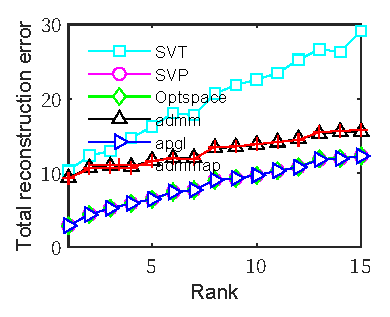
\includegraphics[width=0.45\textwidth]{./assets/fig3-90.eps}}\\
	\caption{ Recovery of an incomplete image with random mask. (The results we reproduced)}
\end{figure}

As shown in picture \ref{fig2}, under different noise levels and different observed ratios, compared with the original image:
\begin{itemize}
	\item Our reproduced (abbreviated as our)SVT algorithm has better overall reconstruction error performance.
	
	\item Our SVP and OptSpace performs better and has similar performance to TNNR-APGL.
	
	\item Our TNNR-ADMM performs similarly to the original image only at low noise levels. However, as the noise level increases, the performance deteriorates faster.
	
	\item Our TNNR-APGL has a similar performance to the original image.
\end{itemize}

As shown in picture \ref{fig3}, under different observed ratios, as the
matrix rank increases, the total reconstruction error becomes larger. Compared with the original image:
\begin{itemize}
	\item Our SVT algorithm has better overall reconstruction error performance at low ranks, and our implementation of the SVT algorithm deteriorates more rapidly as the matrix rank increases.
	
	\item Our SVP and OptSpace performs better and has similar performance to TNNR-APGL.
	
	\item The total reconstruction error of our TNNR-ADMM and TNNR-ADMMAP is relatively large, and the results that are not close to the original work have been reached.
	
	\item Our TNNR-APGL has a similar performance to the original image.
\end{itemize}


\subsection{Real visual data}
In practice, images may be covered with text etc. For color images, the three channels need to be processed separately and combined to get the final result. We use the peak signal-to-noise ratio (PSNR) to evaluate the performance of different methods, assuming the total number of missing pixels is $T$, then
\begin{align*}
	\text{SE} & = error_r^2 + error_g^2 + error_b^2 \\
	\text{MSE} & = \frac{\text{SE}}{3T} \\
	\text{PSNR} & = 10log_{10}(\frac{255^2}{\text{MSE}}).
\end{align*}
where SE denotes the total squared error, MSE denotes the total mean squared error.

\subsubsection{Parameter setting}
In our experiments, the parameters of SVP, SVT, and OptSpace are tuned to achieve the best performance. For TNNR-ADMM, TNNR-APGL and TNNR-ADMMAP, We did not get good results using the original parameters. For TNNR-ADMM, we set $\beta = 10^{-3}$. For TNNR-ADMMAP, we set $\beta_{max} = 10^{10}$, $\kappa = 10^{-3}$, $\rho_0 = 1.1$ in section \ref{random}, and $\rho_0 = 1.01$ in other sections. For TNNR-APGL, the parameter $\lambda$ is empirically set to be $10^{-2}$ in section \ref{text} and $10^{-3}$ in other sections.
  
For the stop conditions of TNNR-ADMM, TNNR-APGL, and TNNR-ADMMAP, we set the tolerance $\epsilon_0$ in Algorithm \ref{algo1} to be $10^{-3}$ and the tolerance $\epsilon$ in Algorithms \ref{algo2}-\ref{algo4} to be $10^{-4}$. Given an incomplete image, for each one of the six algorithms we try all the possible values of $r$ to choose the best results.

\subsubsection{Random mask}
\label{random}
we randomly cover some pixels of an image ($300 \times 300$), and then compare the recovery performance of the six algorithms.The results are shown in Fig,~\ref{fig4} and \ref{fig5}. Naturally, the larger the observed ratio is the better recovery of the image that can be achieved. Form Fig.~\ref{fig5}, we can see that the TNNR-based algorithms can achieve higher PSNR values compared with the other three methods. Compare with the results in the original paper, our SVT recovers images better. And the results of TNNR-APGL are not as expected in the high observed ratio.

\begin{figure}[ht]
	\centering
	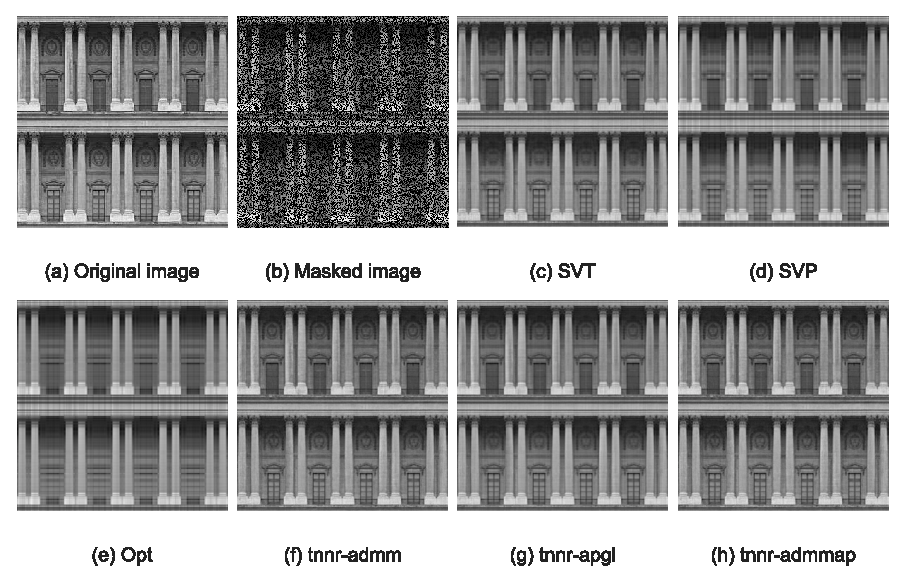
\includegraphics[]{./assets/fig4.eps}
	\caption{The reconstruction error versus the matrix rank ($r_0$) using the synthetic dataset. (The original result of paper)}
	\label{fig4ori}
\end{figure}
\begin{figure}[ht]
	\centering
	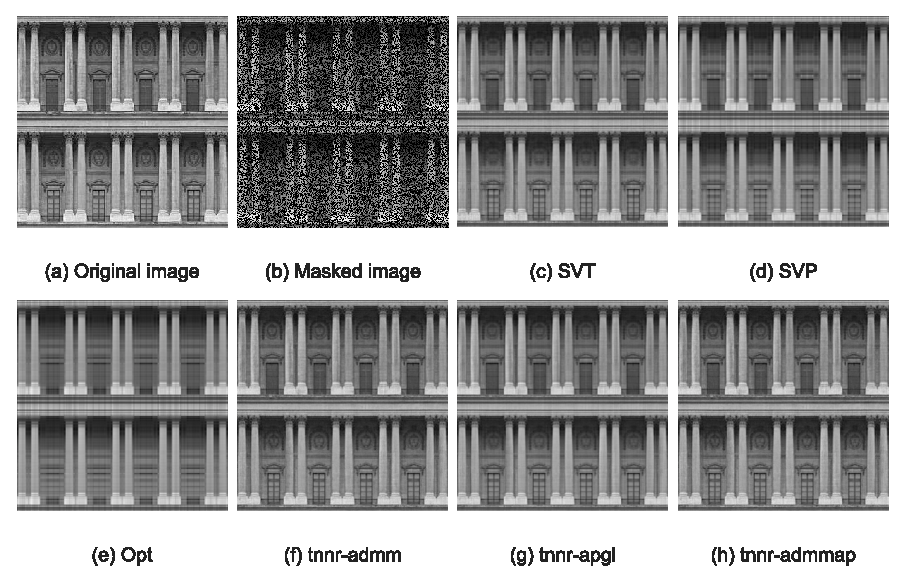
\includegraphics[]{./assets/fig4.eps}
	\caption{The reconstruction error versus the matrix rank ($r_0$) using the synthetic dataset. (The result we reproduced)}
	\label{fig4}
\end{figure}

\begin{figure}[ht]
	\centering
	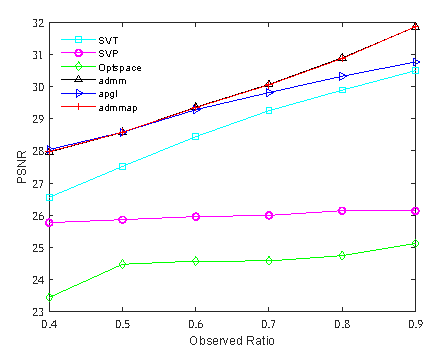
\includegraphics[]{./assets/fig5.eps}
	\caption{The PSNR values of the recovered image under different
		observed ratios (random mask) by all six methods. (The original result of paper)}
	\label{fig5ori}
\end{figure}
\begin{figure}[ht]
	\centering
	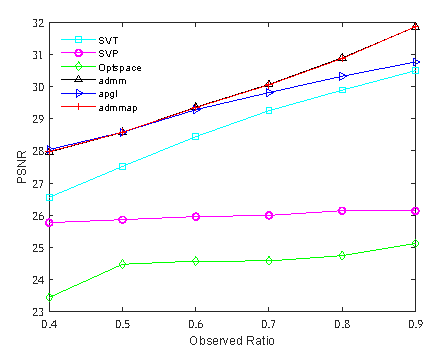
\includegraphics[]{./assets/fig5.eps}
	\caption{The PSNR values of the recovered image under different
		observed ratios (random mask) by all six methods. (The result we reproduced)}
	\label{fig5}
\end{figure}

\subsubsection{Text mask}
\label{text}

Since the text is not random, it may cover important information in the picture, making the text more difficult to remove than pixels. Fig.~\ref{fig7} and Fig.~\ref{fig8} show the experimental results of the six matrix
completion algorithms. Specifically, for the example image
in Fig.~\ref{fig7}, the PSNR values for SVT, SVP, OptSpace, TNNR-
ADMM, TNNR-APGL, and TNNR-ADMMAP are 23.47,
23.47, 22.43, 25.26, 25.26, and 25.27, respectively. And for the
example image in Fig. 8, the PSNR values for SVT, SVP,
OptSpace, TNNR-ADMM, TNNR-APGL, and TNNR-ADMMAP are 21.61, 21.61, 21.95, 23.94, 23.16, and 23.95, respectively. 
From these results we can see that TNNR-ADMM and TNNR-ADMMAP algorithms achieve better performance than the other three matrix completion algorithms. Our TNNR-APGL cannot obtain the same image restoration effect as the original paper.

\begin{figure}[ht]
	\centering
	\includegraphics[]{./assets/fig7.eps}
	\caption{Comparison of matrix completion algorithms for text removal problem. (The original result of paper)}
	\label{fig7ori}
\end{figure}
\begin{figure}[ht]
	\centering
	\includegraphics[]{./assets/fig7.eps}
	\caption{Comparison of matrix completion algorithms for text removal problem. (The result we reproduced)}
	\label{fig7}
\end{figure}

\begin{figure}[ht]
	\centering
	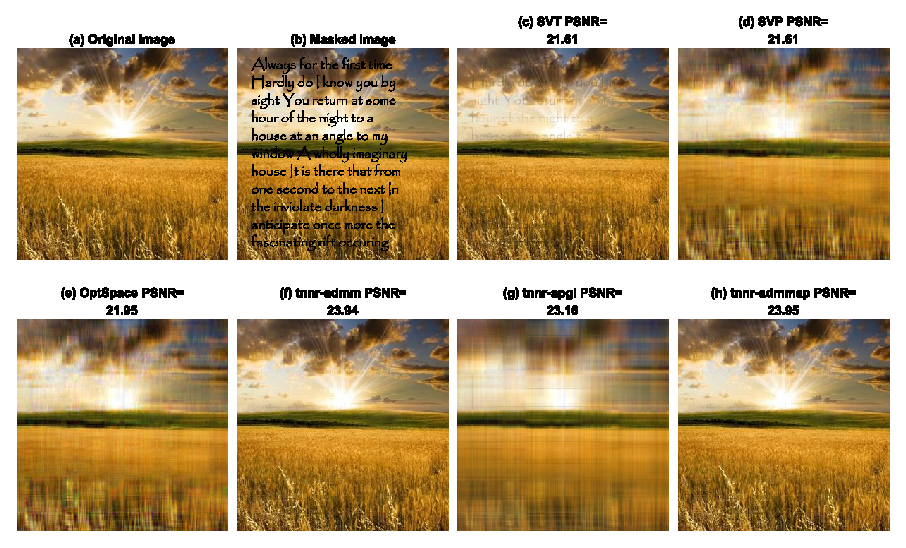
\includegraphics[]{./assets/fig8.eps}
	\caption{Comparison of matrix completion algorithms for text removal problem. (The original result of paper)}
	\label{fig8ori}
\end{figure}
\begin{figure}[ht]
	\centering
	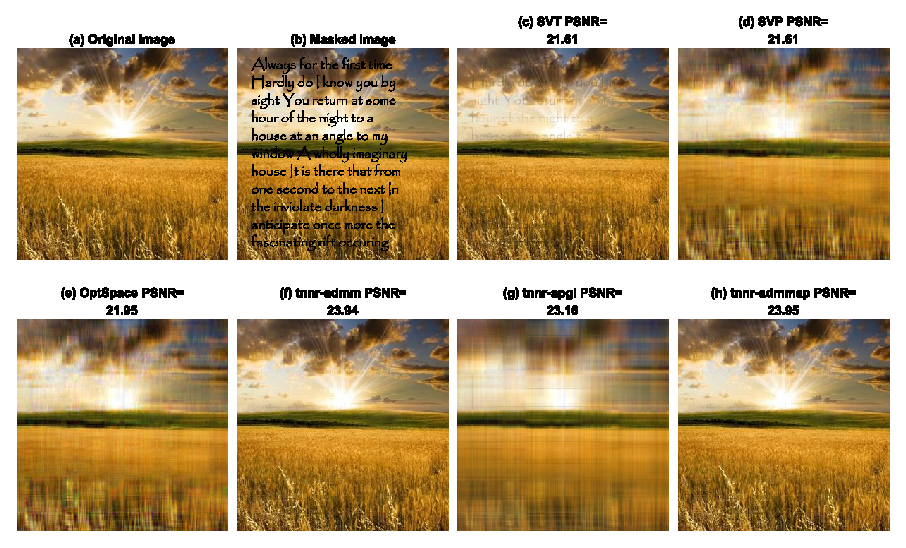
\includegraphics[]{./assets/fig8.eps}
	\caption{Comparison of matrix completion algorithms for text removal problem. (The result we reproduced)}
	\label{fig8}
\end{figure}


\subsubsection{Block mask}
In some situations, Some pixels in the image have been broken. We first mask all these pixels, then we use six matrix completion algorithms to recover these large missing blocks.


\begin{figure}[ht]
	\centering
	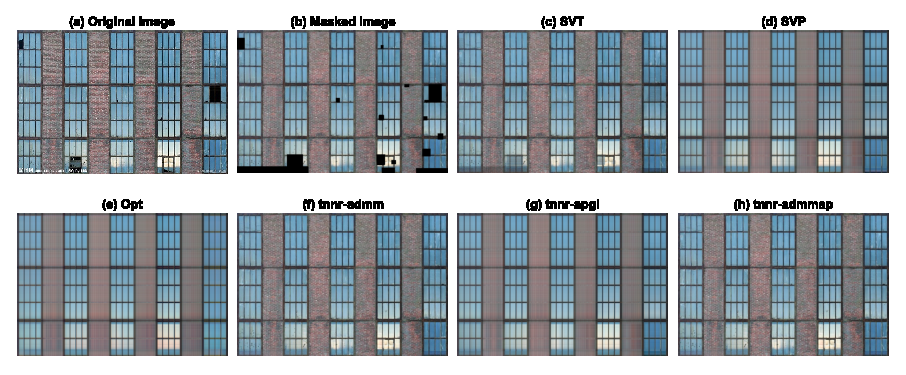
\includegraphics[]{./assets/fig9.eps}
	\caption{Comparison of different methods for recovering missing blocks of
		a natural image. (The original result of paper)}
	\label{fig9ori}
\end{figure}

\begin{figure}[ht]
	\centering
	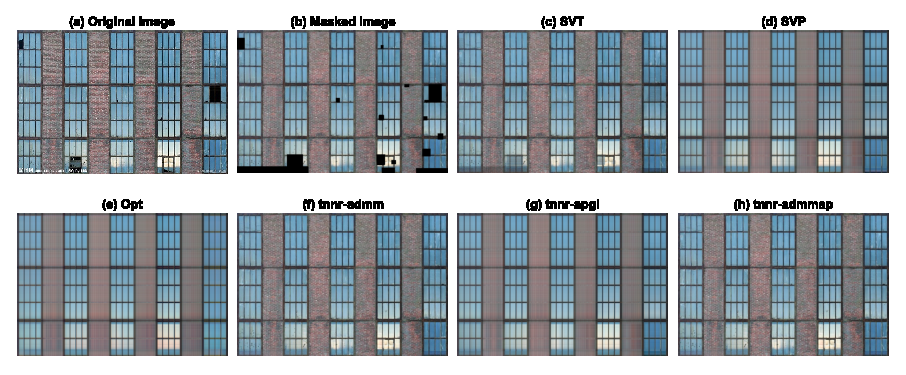
\includegraphics[]{./assets/fig9.eps}
	\caption{Comparison of different methods for recovering missing blocks of
		a natural image. (The result we reproduced)}
	\label{fig9}
\end{figure}

\subsection{Convergence rate and computational cost}


\begin{table}
	\caption{Running time of text masked image recovery}
	\label{rcost}
	\centering
	\begin{tabular}{ccccccc}
		\toprule
		\multirow{2}{*}{Method} & \multicolumn{6}{c}{Observed Ratios} \\
		\cmidrule(r){2-7} 
		& 0.4 & 0.5 & 0.6 & 0.7 & 0.8  & 0.9 \\
		\midrule
		TNNR-ADMM &   &  & & & &   \\
		TNNR-APGL & & & & & &  \\
		TNNR-ADMMAP & & & & & &   \\
		\bottomrule
	\end{tabular}
\end{table}


\section{Conclusion}
\label{s5}




\section*{References}


References follow the acknowledgments. Use unnumbered first-level heading for
the references. Any choice of citation style is acceptable as long as you are
consistent. It is permissible to reduce the font size to \verb+small+ (9 point)
when listing the references.
Note that the Reference section does not count towards the page limit.
\medskip


{\small{}\bibliographystyle{plain}
\bibliography{report}
}{\small\par}

%%%%%%%%%%%%%%%%%%%%%%%%%%%%%%%%%%%%%%%%%%%%%%%%%%%%%%%%%%%%



\appendix


\section{Appendix}
\textit{proof} Theorem~\ref{thm31}

By Von Neumann’s trace inequality, we get
\begin{equation}
	\begin{aligned}
		\text{Tr}(AXB^T) & = \text{Tr}(XB^TA) \\
		& \leq  \sum_{i=1}^{\min(m,n)} \sigma_i(X) \sigma_i(B^TA),
	\end{aligned}
\end{equation}
where $\sigma_1(X) \geq \cdots \geq \sigma_{min(m,n)}(X) \geq 0 $. As $rank(A) = r$ and $rank(B) =r$, so $rank(B^TA) =s \leq r$. For $i \leq s$, $\sigma_i(B^TA) \geq 0$ and $\sigma_i(B^TA)$ is the $i$th eigenvalue of $BB^T=I$. Therefore, $\sigma_i(B^TA) = 1$, for $i=1,2,\dots,s$, and the rest are all 0s. It follows that:
\begin{equation}
	\begin{aligned}
		\sum_{i=1}^{\min(m,n)} \sigma_i(X) \sigma_i(B^TA) & = \sum_{i=1}^{s} \sigma_i(X) \sigma_i(B^TA) + \sum_{i=s+1}^{\min(m,n)} \sigma_i(X) \sigma_i(B^TA) \\
		& = \sum_{i=1}^{s} \sigma_i(X) \cdot 1 + \sum_{i=s+1}^{\min(m,n)} \sigma_i(X) \cdot 0 \\
		& = \sum_{i=1}^{s} \sigma_i(X).
	\end{aligned}
\end{equation}
Since $s \leq r$ and $\sigma_i(X) \geq 0$:
\begin{equation*}
	\sum_{i=1}^s \sigma_i(X)\leq \sum_{i=1}^r \sigma_i(X).
\end{equation*}
Combining inequalities and ,we have 
\begin{equation}
	\text{Tr}(AXB^T) \leq \sum_{i=1}^s \sigma_i(X)\leq \sum_{i=1}^r \sigma_i(X).
\end{equation}


\textit{proof} Equation~\ref{admmx}

Fix $W_k$ and $Y_k$ ,
\begin{equation}
	\label{xeq1}
		X_{k+1} =  \underset{X}{\text{arg min}} \ \Vert X\Vert_* - Tr(A_l W_k B_l^T)    + \frac{\beta}{2}\Vert X-W_k \Vert_F^2 + \text{Tr}(Y_k^T(X-W_k)).
\end{equation}
For the last two terms of \eqref{xeq1},
\begin{equation}
	\label{xeq2}
\frac{\beta}{2}\Vert X-W_k \Vert_F^2 + \text{Tr}(Y_k^T(X-W_k))=  \frac{\beta}{2}\left( \Vert X-W_k \Vert_F^2 + \frac{2}{\beta} \text{Tr}(Y_k^T(X-W_k)) \right).
\end{equation}
Because
\begin{equation*}
	\begin{aligned}
		\Vert X-W_k+\frac{1}{\beta}Y_k \Vert_F^2 & = \text{Tr} \ (X-W_k+\frac{1}{\beta}Y_k)(X-W_k+\frac{1}{\beta}Y_k)^T \\
		& = \text{Tr}(X-W_k)(X-W_k)^T + 2\ \text{Tr}(X-W_k)\frac{1}{\beta}Y_k^T + \frac{1}{\beta^2}\text{Tr} (Y_k Y_k^T) \\
		& = \Vert X-W_k \Vert_F^2 + \frac{1}{\beta^2}\Vert Y_k \Vert_F^2 + \frac{2}{\beta}\text{Tr}(Y_k^T(X-W_k)).
	\end{aligned}
\end{equation*}
For the latter term in parentheses of \eqref{xeq2},
\begin{equation}
	\begin{aligned}
\frac{2}{\beta} \text{Tr}(Y_k^T(X-W_k)) & =  2 \ \text{Tr}(\frac{1}{\beta}Y_k^T(X-W_k)) \\
	& = \Vert X-W_k+\frac{1}{\beta}Y_k \Vert_F^2 - \frac{1}{\beta^2}\Vert Y_k \Vert_F^2 - \Vert X-W_k \Vert_F^2.
\end{aligned}
\end{equation}
Ignoring all constant terms, 
\begin{equation}
\begin{aligned}
	X_{k+1} & =\underset{X}{\text{arg min}}\ L(X,Y_k,W_k,\beta) \\
	& =  \underset{X}{\text{arg min}} \ \Vert X\Vert_* - \text{Tr}(A_l W_k B_l^T)    + \frac{\beta}{2}\Vert X-W_k \Vert_F^2 + \text{Tr}(Y_k^T(X-W_k)) \\
	& = \underset{X}{\text{arg min}} \ \Vert X\Vert_* + \frac{\beta}{2} \Vert X-\left(W_k - \frac{1}{\beta}Y_k \right) \Vert_F^2 - \frac{1}{2\beta} \Vert Y_k \Vert_F^2 \\
	& = \underset{X}{\text{arg min}} \ \Vert X\Vert_* + \frac{\beta}{2} \Vert X-\left(W_k - \frac{1}{\beta}Y_k \right) \Vert_F^2.
\end{aligned} 
\end{equation}
That is 
\begin{equation}
	X_{k+1} = D_{\frac{1}{\rho}}(W_k - \frac{1}{\rho}Y_k).
\end{equation}

\end{document}